\begin{figure*}[t]
  \centering
  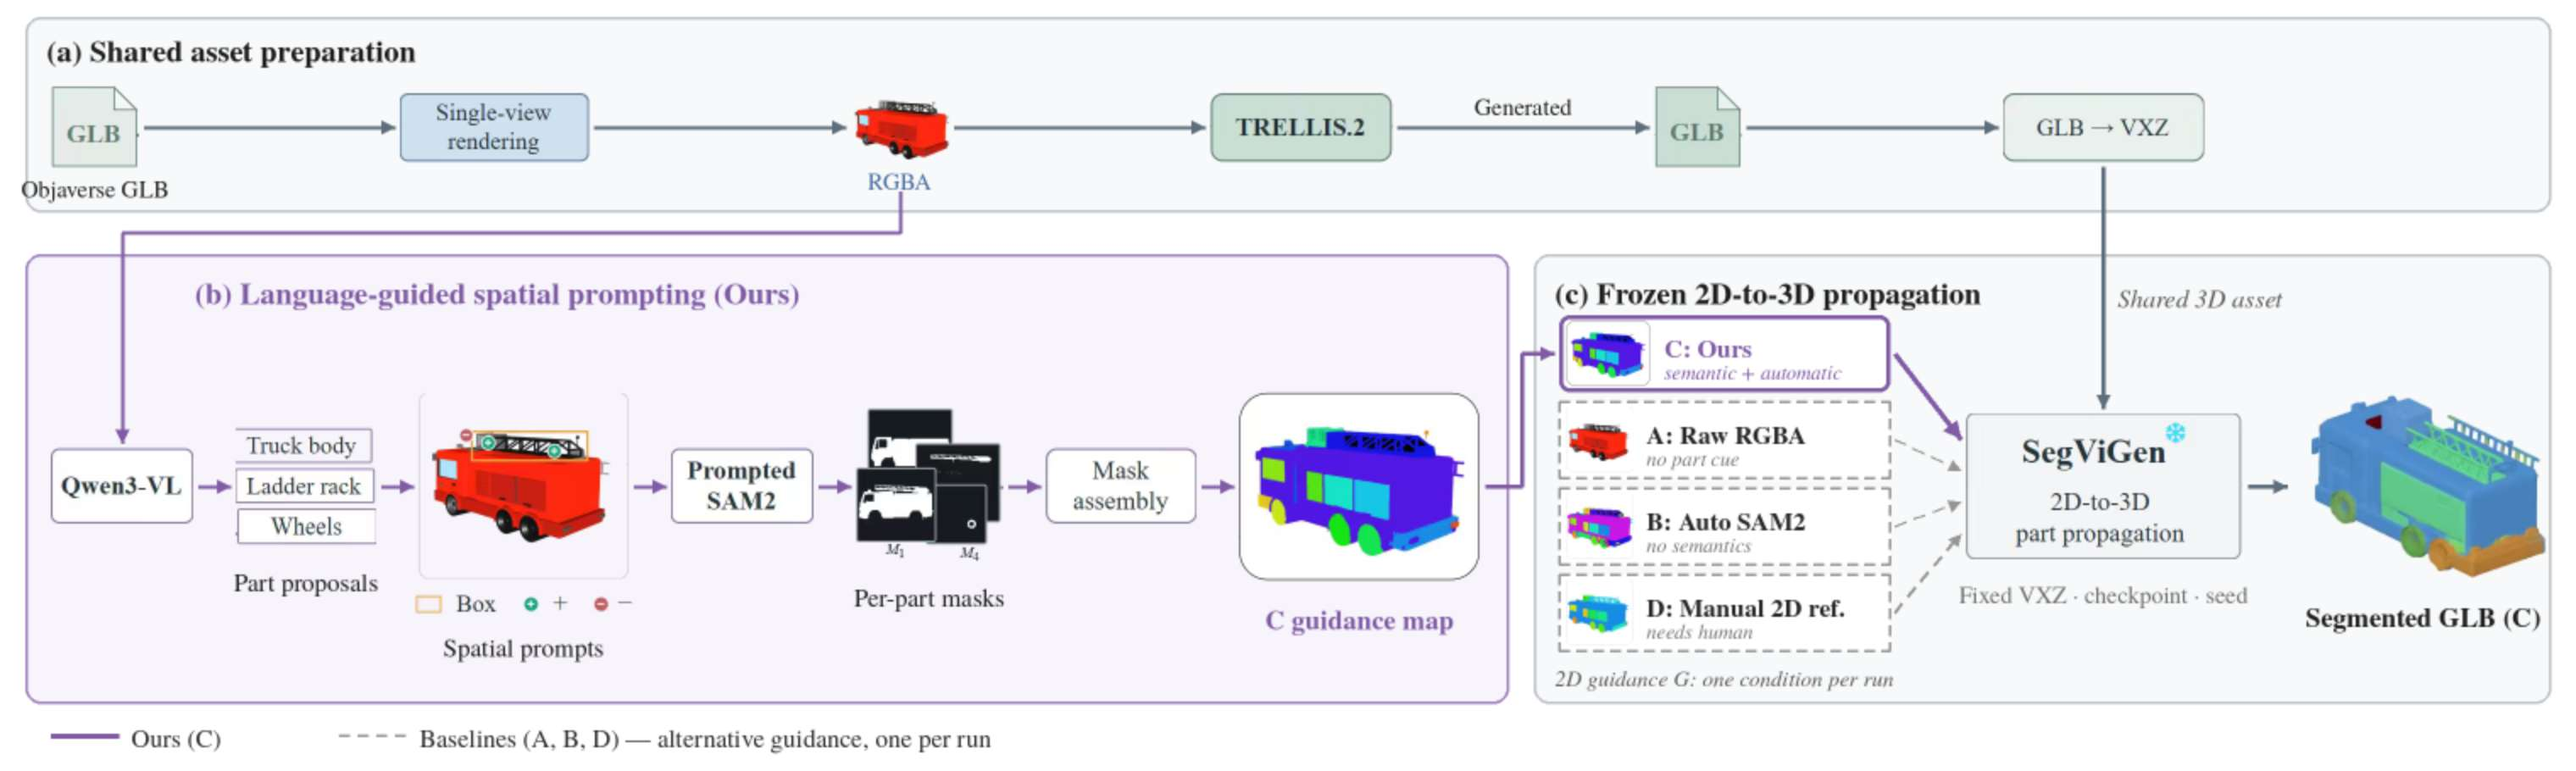
\includegraphics[width=\textwidth]{images/fig1_method.jpg}
  \caption{方法概览。（a）由下载的三维资产渲染输入图像，并构建供比较实验使用的生成资产；（b）Qwen3-VL 提出可见部件及空间提示，SAM2 生成候选掩码，经反馈与融合得到 C 组二维引导；（c）在固定三维资产和推理设置下，每次仅输入一种引导条件，由 SegViGen 输出三维部件分区。A、B、D 是替代引导条件，不与 C 同时输入。图中 ``Shared'' 描述本文采用的受控比较协议，不代表不同条件的最终分割 GLB 相同。候选反馈的具体位置见图\ref{fig:data}。}
  \label{fig:method}
\end{figure*}
